\documentclass{article}
\usepackage{amsmath}
\usepackage{gensymb}
\usepackage{float}
\usepackage[top=1in, bottom=1in, left=1in, right=1in]{geometry}
\usepackage{graphicx}
\usepackage{rotating}
\usepackage{multirow}
\usepackage{amsfonts}
\usepackage{wrapfig}
\usepackage{array}
\usepackage{float}
\usepackage{caption}
\usepackage{subcaption}
\usepackage{ragged2e}
\newcolumntype{K}[1]{>{\centering\arraybackslash}p{#1}}
\usepackage[hidelinks]{hyperref}
\makeatletter
\newcommand*{\rom}[1]{\expandafter\@slowromancap\romannumeral #1@}
\makeatother
\graphicspath{ {Figures/} }
\begin{document}
	\everymath{\displaystyle}
	\begin{titlepage}	 	
		\center
		\text{}\\[3cm]
		\linespread{2}\huge \bfseries MP3: Audio Features
		\center\textsc{\Large ECE 417 Fall 2017}\\[1cm]
		\Large\center\textsc{Weicheng Jiang \\Yuchen Liang\\ Zixu Zhang  }\\[1.4cm]
		\Large \today\\
		\vfill
	\end{titlepage}
	%\tableofcontents\newpage
	\setlength{\baselineskip}{24pt}
	
	\section{Introduction}
	In this MP, we develop a simple speech recognition system which is also used for speaker identification. Data of four people speaking 5 different digits (1, 2, 3, 4 and 5), each for five times are provided for analysis. We first extract and store the audio features from the raw data files. Data files are resized into uniform length and only the left channel of the signals are used. Both the Cepstrum coefficients and the mel-frequency cepstral coefficients (MFCC) are computed and different window sizes are experimented for both Cepstrum and MFCC. All the Cepstra, MFCC and the raw features for each file’s frame are put into a feature vector. Then for each feature vector, we use the nearest neighbor (NN) algorithm using leaving-N-out strategy for both speech and speaker recognition. Results of the performances of our speech and speaker recognition system are then generated for comparison. 

	\section{Method}
	\subsection{Ceptrum Analysis}
	Ceptrum is defined as the inverse Fourier transform of the log spectrum of a signal, as it can be written as
	$$
	\hat{s}[q]=\mathcal{F}^{-1}\{\ln |\mathcal{F}[s(t)]|\}
	$$
	The speech signal, for example, is the convolution of the excitation signal $e(t)$ by vocal fold and vocal tract transfer function $h(t)$, such that 
	$
	s(t)=h(t)*e(t)
	$.
	Therefore, the cepstrum of voice signal becomes the sum of cepstrums of excitation signal and the impluse response of vocal tract transfer function.
	$$
	\hat{s[q]}=\mathcal{F}^{-1}\{\ln |\mathcal{F}[h(t)]|+\ln |\mathcal{F}[e(t)]|\}=\hat{e}[q]+\hat{h}[q]
	$$
	The idea behind the cepstrum is that the inverse Fourier transform measures the inverse frequency of those peaks in spectrum, and transfer the signal from frequency domain to quefrency domain. Moreover, the log magnitude of spectrum compress peaks in spectrum, and makes the cepstrum analysis easier to detect sequential periodic. The nature of human speech is that the spacing between harmonics of vocal folds excitation, $F(0)$, has low frequency, while the spacing between vocal tract resonances, format frequency, are higher than $F(0)$. Therefore, excitation signals will have high quefrency, while the vocal tract transfer function will have low quefrency. With cepstrum analysis, we can separate excitation and vocal tract transfer function by a windows function $w[q]$.
	$$
	\hat{h}[q]\approx w[q]\hat{s}[q]~	\hat{e}[q]\approx(1- w[q])\hat{s}[q]
	$$
	In this MP, we first find out the number of discrete Fourier transform as $NFFT$, which should be a number with power of 2, and larger than the size of window $NW$. After preemphasis filtering the signal in line 15, we divide the single voice signal into frames. This process is done by function \texttt{sig2frames.m}, and the output will be $NF$ frames with length $NW$. For each frame, the last 10\% of data will overlap the next frame.\\
	A cepstrum analysis of each frame is done in line 24 of \texttt{cepstrum.m} following equation 1. Since the higher order of ceptral coefficient is two small, we select first $NNC$ ceptral coefficient, and reshape cepstrums of each frames into a single column vector.
	
	
	
	
	\subsection{MFCC}
	The discrete cosine transform (DCT) is half of the real symmetric IFFT of a real symmetric signal. Suppose we define spectral distance $C_k=\ln|S(\frac{(0.5+k)F_s}{N})|$, and $c[n]=M\hat{s}[n],~n\geq1$, where $M=N/2$. In this case, we can define type II DCT as:
	\begin{equation}
	c[n]=\frac{N}{2}\mathcal{F}^{-1}(\ln|S(f)|)=\sum_{k=0}^{M-1}C_k\cos(\frac{\pi(n+0.5)n}{M})
	\end{equation}
	In practice, we can approximate the spectral distance as the FFT coefficient, $C_k\approx\ln|S(\frac{kF_s}{N})|$. By Parseval's theorem, $c[0]=\sum_{k=0}^{N-1}C_k$, which is the average log magnitude of the spectrum. \\
	The mel-frequency cepstrum coefficients (MFCC) is a different method for recognition. The key difference with merely cepstrum coefficients (CC) is that it uses a mel scale rather than a hertz scale, which is adapted from human auditory perception system and is nonlinear in frequency. Mathematically, after achieving the CC of each frame, rather than finding the smoothing version, we pass it through an array of filters H (the properties of which is listed below). This is done by computing $Y = HWX$ where each column of X is the \texttt{NFFT}-point fft of each frame. $W\in\mathbb{R}^{M\times NFFT}$ is constructed to get rid of the aliasing artifact from log spectrum, and it has a $M\times M$ identity submatrix along with a $M\times M-2$ zero submatrix, where $M=\frac{NFFT}{2}+1$. In Matlab, it is constructed in line 62, with simply code \texttt{W=eye(M,NFFT);}. Intuitively, MFCC compresses high frequencies and differentiates at speech-related frequencies, so it can differentiate speeches more correctly. $H$ is the mel filterbank matrix, whose rows are filters centered at $M$ different frequency points such that each window $W_k$ is a shifted triangular function with peak frequency $f_k$.The magnitude of each window vanishes at its neighbor’s peak frequency as $W_k[f_{k-1}] = W_k[f_{k+1}] = 0$. In MFCC, the first peak frequency $f_0 = 0$, while the last peak frequency $f_M = F_s/2$. The peak frequencies $f_k$ distribute linearly on the mel scale. This means $delta(m) = m_k - m_{k-1} = (m_M - 0) / M = C$, which is a constant, and $m_k \approx  2593\log_{10}(1+\frac{f}{700})$
	
	
	
	
	
	\subsection{K-NN}
	The files \texttt{knn.m} and \texttt{findlabel.m} contains all of the calculation for the kNN classifier. It classifies the test data as the same label that appears for its nearest $k$ neighbors by finding Euclidean distance squared between test data and train datas.
	For a test data $\mathbf{x}_\text{test}$, we want to find $k$ indexes that give the k smallest $d_2(\mathbf{x}_\text{test},\mathbf{x_i})^2$ value, where $1\leq i\leq M$. Then we label $\mathbf{x}_\text{test}$ as the label $l_m$ that appear the most times in k nearest neighbor.\\
	The difference between the K-NN function with the one we implemented before is that we have two modes of recognition for both speech and speaker. From line 15 to 20, we have the K-NN for speech recognition, which takes in 75 sets of training data spoken by different speakers other than the speaker of test data. It will call speech recognition mode of label finer in line 9 to 20 of \texttt{findLabel.m}. The line 22 to 32 in the function \texttt{knn.m} is the K-NN for speaker recognition. It will takes 80 sets of training data with different words other than the one in the test data. Then, speaker label finder, from line 23 to 33 in \texttt{findLabel.m}, is invoked by this function.


	
	
	\section{Results}
	
	We conduct speech recognition experiments with raw voice features, cepstrums, and MFCC of features by both 1-NN and 5-NN classifiers. Their results are tabulted in Table \ref{tab:speech_cepstrum} and \ref{tab:speech_mfcc}. 
	\begin{table}[H]
		\centering
		\caption{1-NN and 5-NN Speech Recognition Results with Ceptrum}
		\label{tab:speech_cepstrum}
		\begin{tabular}{c|K{1cm}|K{1.4cm}|K{1.4cm}|K{1.4cm}|c|K{1.4cm}|K{1.4cm}|K{1.4cm}|K{1.4cm}|}
			\cline{2-5} \cline{7-10}
			& \multicolumn{4}{c|}{\textbf{1-NN}}     &  & \multicolumn{4}{c|}{\textbf{5-NN}}     \\ \cline{1-5} \cline{7-10} 
			\multicolumn{1}{|c|}{Digit} & Raw & W=100 & W=500 & W=10000 &  & Raw & W=100 & W=500 & W=10000 \\ \cline{1-5} \cline{7-10} 
			\multicolumn{1}{|c|}{D1}    & 0   & 70    & 65    & 20      &  & 0   & 85    & 65    & 25      \\ \cline{1-5} \cline{7-10} 
			\multicolumn{1}{|c|}{D2}    & 30  & 45    & 50    & 70      &  & 35  & 45    & 55    & 45      \\ \cline{1-5} \cline{7-10} 
			\multicolumn{1}{|c|}{D3}    & 15  & 70    & 65    & 70      &  & 5   & 50    & 45    & 60      \\ \cline{1-5} \cline{7-10} 
			\multicolumn{1}{|c|}{D4}    & 50  & 70    & 65    & 65      &  & 40  & 60    & 55    & 60      \\ \cline{1-5} \cline{7-10} 
			\multicolumn{1}{|c|}{D5}    & 0   & 60    & 70    & 30      &  & 5   & 70    & 80    & 45      \\ \cline{1-5} \cline{7-10} 
			\multicolumn{1}{|c|}{Ave}   & 19  & 63    & 63    & 51      &  & 17  & 62    & 60    & 47      \\ \cline{1-5} \cline{7-10} 
		\end{tabular}
	\end{table}


	\begin{table}[H]
		\centering
		\caption{1-NN and 5-NN Speech Recognition Results with MFCC}
		\label{tab:speech_mfcc}
		\begin{tabular}{c|K{1cm}|K{1.4cm}|K{1.4cm}|K{1.4cm}|c|K{1.4cm}|K{1.4cm}|K{1.4cm}|K{1.4cm}|}
			\cline{2-5} \cline{7-10}
			& \multicolumn{4}{c|}{\textbf{1-NN}}     &  & \multicolumn{4}{c|}{\textbf{5-NN}}     \\ \cline{1-5} \cline{7-10} 
			\multicolumn{1}{|c|}{Digit} & Raw & W=100 & W=500 & W=10000 &  & Raw & W=100 & W=500 & W=10000 \\\cline{1-5} \cline{7-10} 
			\multicolumn{1}{|c|}{D1}  & 0   & 55    & 60    & 35      &                       & 0   & 85    & 70    & 25      \\ \cline{1-5} \cline{7-10} 
			\multicolumn{1}{|c|}{D2}  & 30  & 65    & 90    & 90      &                       & 35  & 65    & 90    & 80      \\ \cline{1-5} \cline{7-10} 
			\multicolumn{1}{|c|}{D3}  & 15  & 95    & 100   & 90      &                       & 5   & 90    & 95    & 90      \\ \cline{1-5} \cline{7-10} 
			\multicolumn{1}{|c|}{D4}  & 50  & 75    & 75    & 60      &                       & 40  & 55    & 65    & 60      \\ \cline{1-5} \cline{7-10} 
			\multicolumn{1}{|c|}{D5}  & 0   & 80    & 90    & 50      &                       & 5   & 85    & 80    & 65      \\ \cline{1-5} \cline{7-10} 
			\multicolumn{1}{|c|}{Ave} & 19  & 74    & 83    & 65      &                       & 17  & 76    & 80    & 64      \\ \cline{1-5} \cline{7-10} 
		\end{tabular}
	\end{table}

	\justify In addition to speach recognition, we also perform speaker recognition with raw voice features, cepstrums, and MFCC of features by both 1-NN and 5-NN classifiers. We present experiment results in Table \ref{tab:speaker_cepstrum} and \ref{tab:speaker_mfcc}.
	
	\begin{table}[H]
		\centering
		\caption{1-NN and 5-NN Speaker Recognition Results with Ceptrum}
		\label{tab:speaker_cepstrum}
		\begin{tabular}{c|K{1cm}|K{1.4cm}|K{1.4cm}|K{1.4cm}|c|K{1.4cm}|K{1.4cm}|K{1.4cm}|K{1.4cm}|}
			\cline{2-5} \cline{7-10}
			& \multicolumn{4}{c|}{\textbf{1-NN}}     &  & \multicolumn{4}{c|}{\textbf{5-NN}}     \\\cline{1-5} \cline{7-10} 
			\multicolumn{1}{|c|}{Digit} & Raw & W=100 & W=500 & W=10000 &  & Raw & W=100 & W=500 & W=10000 \\ \cline{1-5} \cline{7-10} 
			\multicolumn{1}{|c|}{A}   & 8   & 52    & 60    & 56      &  & 0   & 52    & 68    & 48      \\ \cline{1-5} \cline{7-10} 
			\multicolumn{1}{|c|}{B}   & 76  & 60    & 52    & 88      &  & 84  & 52    & 60    & 76      \\ \cline{1-5} \cline{7-10} 
			\multicolumn{1}{|c|}{C}   & 36  & 20    & 32    & 52      &  & 12  & 16    & 12    & 48      \\ \cline{1-5} \cline{7-10} 
			\multicolumn{1}{|c|}{D}   & 16  & 40    & 32    & 40      &  & 0   & 36    & 28    & 52      \\ \cline{1-5} \cline{7-10} 
			\multicolumn{1}{|c|}{Ave} & 34  & 43    & 44    & 59      &  & 24  & 39    & 42    & 56      \\ \cline{1-5} \cline{7-10}
		\end{tabular}
	\end{table}


	\begin{table}[H]
		\centering
		\caption{1-NN and 5-NN Speaker Recognition Results with MFCC}
		\label{tab:speaker_mfcc}
		\begin{tabular}{c|K{1cm}|K{1.4cm}|K{1.4cm}|K{1.4cm}|c|K{1.4cm}|K{1.4cm}|K{1.4cm}|K{1.4cm}|}
			\cline{2-5} \cline{7-10}
			& \multicolumn{4}{c|}{\textbf{1-NN}}     &  & \multicolumn{4}{c|}{\textbf{5-NN}}     \\ \cline{1-5} \cline{7-10} 
			\multicolumn{1}{|c|}{Digit} & Raw & W=100 & W=500 & W=10000 &  & Raw & W=100 & W=500 & W=10000 \\\cline{1-5} \cline{7-10} 
		\multicolumn{1}{|c|}{A}   & 8   & 40    & 60    & 56      &  & 0   & 60    & 64    & 60      \\ \cline{1-5} \cline{7-10} 
		\multicolumn{1}{|c|}{B}   & 76  & 60    & 84    & 76      &  & 84  & 52    & 76    & 80      \\ \cline{1-5} \cline{7-10} 
		\multicolumn{1}{|c|}{C}   & 36  & 40    & 36    & 64      &  & 12  & 52    & 52    & 44      \\ \cline{1-5} \cline{7-10} 
		\multicolumn{1}{|c|}{D}   & 16  & 16    & 32    & 56      &  & 0   & 16    & 28    & 40      \\ \cline{1-5} \cline{7-10} 
		\multicolumn{1}{|c|}{Ave} & 34  & 39    & 53    & 63      &  & 24  & 45    & 55    & 56      \\ \cline{1-5} \cline{7-10} 
		\end{tabular}
	\end{table}

	\justify In order to have a better visualization of the relationship between accuracy and different window sizes and methods, we show the total accuracy of speech and speaker recognition with respect of window size in Figure \ref{fig:speech} and \ref{fig:speaker}.
	\begin{figure}[H]
		\centering
		\begin{subfigure}[t]{0.49\textwidth}
			\centering
			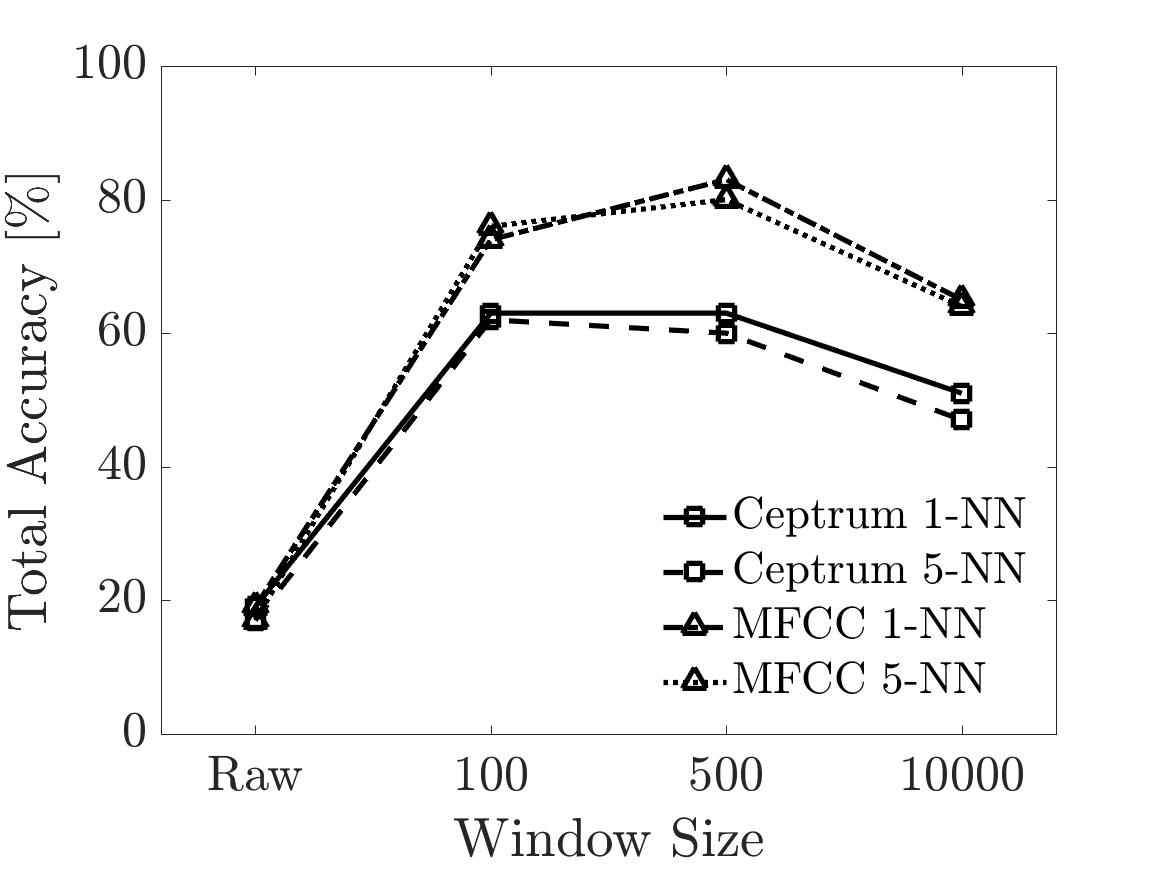
\includegraphics[width=\textwidth]{speech_accuracy}
			\caption{Speech Recognition Accuracy versus Window Size}
			\label{fig:speech}
		\end{subfigure}~
		%
		\begin{subfigure}[t]{0.49\textwidth}
			\centering
			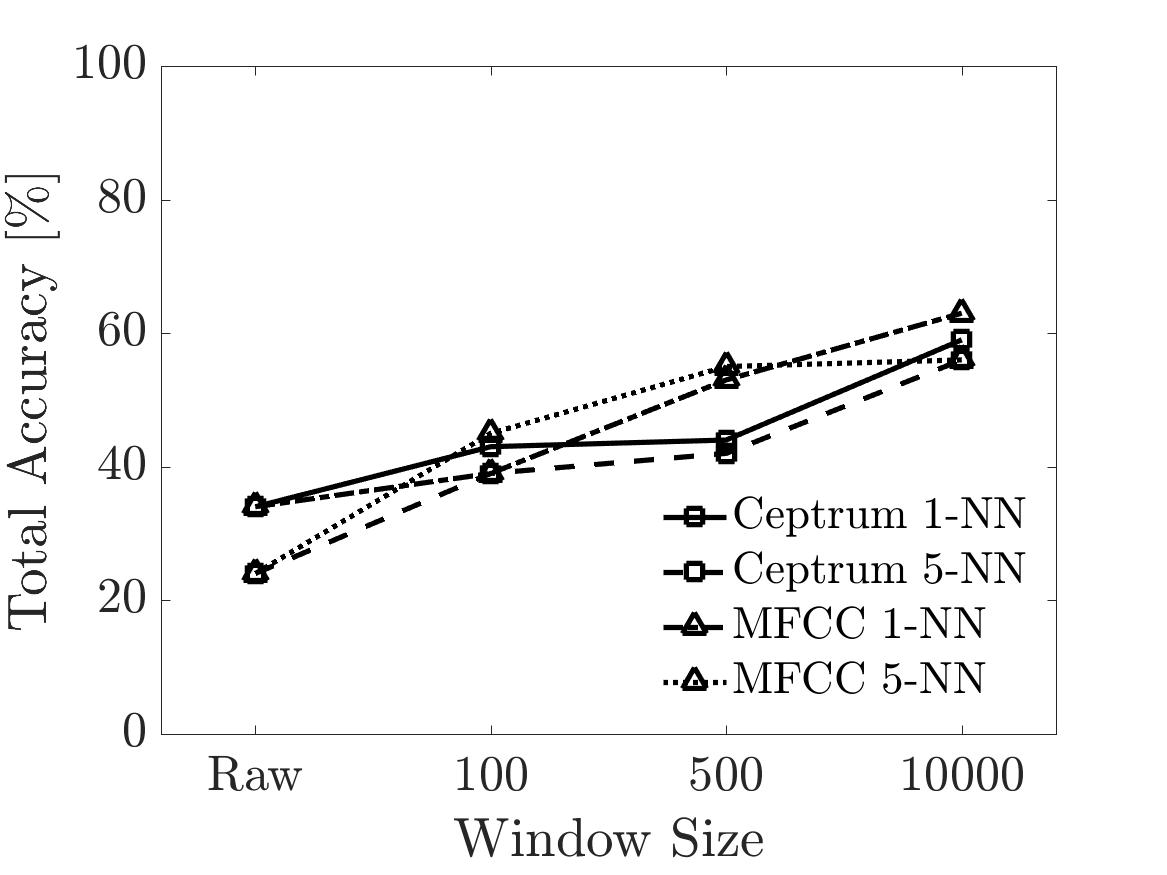
\includegraphics[width=\textwidth]{speaker_accuracy}
			\caption{Speaker Recognition Accuracy versus Window Size}
			\label{fig:speaker}
		\end{subfigure}
	
	\caption{Speech and Speaker Recognition Experiments with Raw, Ceptrum and MFCC Features}
		
	\end{figure}
	
	\section{Discussion}
	There are two observations for speech recognition: 1) MFCC features perform better than simple cepstrum coefficients at any of the window size, and 2) either too small or large window sizes will decrease the accuracy of recognition. The first part is probably because MFCC uses a mel scale rather than a hertz scale, which is nonlinear in frequency. It compresses high frequencies and differentiates at speech-related frequencies, so it can differentiate speeches more correctly. At small window sizes, an increase in window size can dissect the phonemes better thus introducing phoneme-related features, but a too large window (10000 above) would provide too little feature for classification.\\
	For the speaker recognition, MFCC does a little better than cepstrum, but the difference is tiny. In contrast, an increase in window size constantly increases the accuracy of speaker recognition. This is probably the result of the cepstrum coefficients we choose. Different from speech recognition, the spacing between harmonics, $F_0$, which identify the speaker of an audio lies in the high quefrency cepstrum. Shrinking the window size emphasize low quefrency cepstrum (since it has less “noise” in the spectrum) that is easy for smoothing, but it makes the detection of frequency-varying $F_0$ harder. Therefore, whether to use CC or MFCC does not make much difference, as we always choose the first 12 cepstrum coefficients, though increasing window size makes $F_0$ easier to detect. 
	
		
		

\end{document}
